%% 
%% Copyright 2007-2020 Elsevier Ltd
%% 
%% This file is part of the 'Elsarticle Bundle'.
%% ---------------------------------------------
%% 
%% It may be distributed under the conditions of the LaTeX Project Public
%% License, either version 1.2 of this license or (at your option) any
%% later version.  The latest version of this license is in
%%    http://www.latex-project.org/lppl.txt
%% and version 1.2 or later is part of all distributions of LaTeX
%% version 1999/12/01 or later.
%% 
%% The list of all files belonging to the 'Elsarticle Bundle' is
%% given in the file `manifest.txt'.
%% 
%% Template article for Elsevier's document class `elsarticle'
%% with harvard style bibliographic references

%\documentclass[preprint,12pt,authoryear]{elsarticle}

%% Use the option review to obtain double line spacing
%% \documentclass[authoryear,preprint,review,12pt]{elsarticle}

%% Use the options 1p,twocolumn; 3p; 3p,twocolumn; 5p; or 5p,twocolumn
%% for a journal layout:
%% \documentclass[final,1p,times,authoryear]{elsarticle}
%% \documentclass[final,1p,times,twocolumn,authoryear]{elsarticle}
%% \documentclass[final,3p,times,authoryear]{elsarticle}
%% \documentclass[final,3p,times,twocolumn,authoryear]{elsarticle}
%% \documentclass[final,5p,times,authoryear]{elsarticle}
\documentclass[final,5p,times,twocolumn,authoryear, 10pt]{elsarticle}
\makeatletter
\def\ps@pprintTitle{%
 \let\@oddhead\@empty
 \let\@evenhead\@empty
 \def\@oddfoot{}%
 \let\@evenfoot\@oddfoot}
\makeatother

%% For including figures, graphicx.sty has been loaded in
%% elsarticle.cls. If you prefer to use the old commands
%% please give \usepackage{epsfig}

%% The amssymb package provides various useful mathematical symbols
\usepackage{amssymb}
\usepackage{amsmath}
\usepackage{lipsum}
\usepackage{algorithm}
\usepackage{algpseudocode}
\usepackage[labelfont=bf]{caption}
\usepackage{float}
\usepackage{listings}
\usepackage{fancyvrb}
\usepackage{dsfont}
\usepackage{relsize}

%% The amsthm package provides extended theorem environments
%% \usepackage{amsthm}

%% The lineno packages adds line numbers. Start line numbering with
%% \begin{linenumbers}, end it with \end{linenumbers}. Or switch it on
%% for the whole article with \linenumbers.
%% \usepackage{lineno}
\usepackage{hyperref}
\hypersetup{
    colorlinks=true,
    linkcolor=blue,
    filecolor=magenta,      
    urlcolor=cyan,
    pdftitle={Overleaf Example},
    pdfpagemode=FullScreen,
}

\setcitestyle{square}
\setcitestyle{numbers}


\newcommand{\dsum}[2]{\mathlarger{\sum}_{#1}^{#2}}
\newcommand{\bgc}{\begin{center}}
\newcommand{\enc}{\end{center}}
\newcommand{\Lg}{\mathcal{L}}
\newcommand\mycaption[1]{{\footnotesize #1}}
\newcommand\repo[1]{https://github.com/siddha20/CSCI4320-Project/tree/master/#1}
\newcommand{\C}[1]{\lstinline{#1}}
\lstset{
  basicstyle=\ttfamily,
  columns=fullflexible,
  keepspaces=true,
}

\begin{document}

\begin{frontmatter}

\title{Simulating a Large-Scale and Secure Voting System}


\author{Siddha Kilaru}
\ead{kilars2@rpi.edu}
\author{Alex Riddle}
\ead{riddla@rpi.edu}

\address{Rensselaer Polytechnic Institute, Troy, NY}


\begin{abstract}
%% Text of abstract
This paper proposes an approach to simulate a large-scale and secure voting
system. The process involves two main steps: generating encrypted votes and
then tallying them up to determine the preferred candidate. The project
leverages high-performance computing as the vote generation process can be
distributed across multiple compute nodes to scale up voter counts. Moreover,
the paper describes how the vote generation algorithm can be used in simulating
election outcomes using Monte Carlo. Furthermore, the safeness of a fully
digital voting system is also investigated in the paper. The paper explores the
effectiveness of standard encryption and cryptography algorithm in ensuring
voter privacy and integrity. We find that parallel computing massively helps in
generating large amounts of voter data and also provides a noticeable speedup
in tallying up votes and Monte Carlo simulations. Additionally,
\textbf{INCOMPLETE}.


\end{abstract}

\begin{keyword}
%% keywords here, in the form: keyword \sep keyword
Distributed Computing \sep Voting Systems \sep Monte Carlo \sep Cryptography
\sep Encryption Algorithms \sep Graph Algorithms \sep Algorithmic Game Theory

%% PACS codes here, in the form: \PACS code \sep code

%% MSC codes here, in the form: \MSC code \sep code
%% or \MSC[2008] code \sep code (2000 is the default)

\end{keyword}


\end{frontmatter}
{ \hypersetup{hidelinks} \tableofcontents}

%% \linenumbers

%% main text
\section{Introduction}
\label{introduction}

In this paper, we want to simulate a large-scale and safe voting system. Our
paper can be separated into two distinct steps. The first step is creating
votes. In the real world, during an election day, a large population submits
ballots containing rankings of their preferred candidates. We aim to simulate
this by generating a file containing a list of candidate rankings equal to the
number of voters. Note that in the real world, this large list of rankings is
not localized to just one location (it would be spread across states, for
example); however, for our model, we assume that all the votes have been
gathered in the same place. After all the votes have been generated, they are
then encrypted. The second stage of the experiment is tallying up the number of
votes to find the preferred candidate. To do this, the encrypted votes must
first be decrypted, and then in order to find the preferred candidate
efficiently, we employ the Schulze method.

So how exactly does our project relate to high-performance computing? First,
generating candidate listings is not exactly a trivial task. The population of
the US is currently over 300 million, and if each voter is asked to rank their
top 20 candidates, repeated generations can take time. In this paper, we
develop a way to distribute this generation across multiple compute nodes in
order to scale up our vote counts to large numbers. Moreover, we make use of
the Fisher-Yates shuffle algorithm to efficiently generate unbiased
permutations of candidate rankings. In addition to generating unbiased
permutations, we experiment with biased permutations using custom distributions
and make use of Monte Carlo simulations to see how candidate rankings are
affected. 

After the votes are generated, we use AES to encrypt the votes in blocks and
distribute the blocks across compute nodes. AES is a block cipher, and block
ciphers need to use modes to work securely. In particular, we are going to use
the counter (CTR) mode of AES, which allows us to determine the key for any
block of the large data, thus allowing us to parallelize the encryption and
decryption process. Each node receives a chunk of the larger file, and each
rank decrypts/encrypts the blocks in parallel using threads as well, which
gives us two "levels" of parallelization for this process. We will also test
using various key sizes of AES, starting with 128 and going up to 256. The
larger the key size, the more expensive the encryption is, though the block
sizes remain the same. After AES encryption, we then hash (SHA-1) the encrypted
votes in blocks and also spread the workload across compute nodes. The hashing
is used to compare the received encryption to the original one to ensure no
votes were modified.

Finally, the decrypted votes are tallied up. This tallying process requires
creating a graph and running a graph algorithm, which we parallelize. The main
advantage a high computing platform gives us is to scale voter numbers to
extremely large numbers. Additionally, our parallel voting and encryption
algorithms can serve as benchmarks for other supercomputing platforms as they
are easily standardizable.

\section{Generating Votes}
\label{Generating Votes}

\subsection{A Simple Vote Model}
\label{A Simple Vote Model}
A vote in our experiment consists of a preferential ordering of candidates. So
given a set of candidates $C = \{c_1, c_2, c_3, \ldots, c_n\}$ where $n \geq
1$, we generate a permutation $P = \{c^*_1, c^*_2, c^*_3, \ldots, c^*_n\}$ of
$C$ according to some distribution. Moreover, for some for some $i < j$ where
$i, j \in [1, n]$, $c^*_i$ is strictly preferred to candidate $c^*_j$. For
simplicity's sake, our model does not account for any ties, so if a voter
equally prefers two or more candidates, we do not take that into account.

One of our main goals is to generate a number of votes $m \gg 1$ in very large
quantities. Doing so allows us to run accurate Monte Carlo simulations and also
test the robustness of our usage of SHA-1 and AES that create certain safety
measures for the votes. The best way to do this is by storing the vote data in
files rather than depending on program memory. There are two main reasons for
this. First, storing the data in files is much more efficient for repeated
access. Generating votes every time an executable starts is not practical and
counter-productive. Second, storing the votes in files allow us to separate the
processes of the voting process. That is, we use an executable to generate and
encrypt votes into a file and then another executable to read in, decrypt
votes, and generate a candidate ranking. Also, using files is much more
convenient for repeated access. 

\subsection{Vote Generation Algorithm}
\label{Vote Generation Algorithm}
We distribute the workload across several compute nodes (ranks) to generate
votes using MPI. Also, we make use of MPI parallel I/O so each rank can write
to a file in parallel as well. The main algorithm for this process is given
below:
\begin{algorithm}[H]
    \caption{Parallel Vote Generation}\label{alg:cap}
    \begin{algorithmic}[1]
    \Procedure{VoteGen}{$rank$, $startId$, $endId$}
    \For{$i\gets startId, endId$}
        \State $voteSequence$.Append(RandomPermutation())
    \EndFor

    \State $size$ $\gets$ SizeOf($voteSequence$)
    \State $allSizes$ $\gets$ AllGather($size$) \Comment{Sizes for all ranks.}
    \State $cursorPos$ $\gets$ CumulativeSum($AllSizes$)
    \State MPIFileSeek$(cursorPos[rank])$
    \State MPIFileWriteAll$(voteSequence)$
    \EndProcedure
    \end{algorithmic}
\end{algorithm}

This algorithm is active in every single rank. The inputs to the algorithm are
$rank$, $startId$, and $endId$. Different $startId$s and $endId$s are passed to
the ranks, representing the section of votes each rank is responsible for
generating and writing. They are calculated by partitioning the total number of
voters across ranks and then carefully assigning the bounds for each rank. This
partition can be calculated ahead of time because the total number of desired
votes is passed to the executable as an argument. The first part of the
algorithm is to generate the vote sequence. To do this, we loop across the
rank's assigned range (prescribed by $startId$ and $endId$) and append to
$voteSequence$, which is a buffer that contains the vote sequences for all the
assigned ids. Since the buffer sizes are not known until they are fully
generated, the ranks need to share the buffer sizes with each other to write to
the file in the correct place. Consequently, the next step is to accurately
assign cursor positions for each rank; in parallel I/O, it is very important
that alignment across different ranks is perfect; otherwise, you risk
overwriting data. To achieve this, the buffer sizes are shared across all the
ranks with each other and stored in $allSizes$. Using that array, we then
generate the array $cursorPos$, which is just the cumulative sum. Finally,
using $cursorPos[rank]$, which is the correct cursor position for $rank$, the
contents of the buffer ($voteSequence$) can be written to the file.
Specifically, we use \C{MPI_File_seek} to move the file cursor and use the
collective write operation \C{MPI_File_write_all} to write the contents of the
buffer to the file:
\begin{center}
    \begin{BVerbatim}
MPI_File_seek(fh, cursor_pos[rank - 1], 
              MPI_SEEK_SET);
MPI_File_write_all(fh, vote_sequence, 
                   size, MPI_CHAR, NULL);
    \end{BVerbatim}
\end{center}
This is different than using independent I/O, where every rank writes to a file
independently; collective I/O mandates that all process are writing to a file
at the same time, which allows MPI to perform certain optimizations making it
much faster overall \cite{pacheco}. Moreover, by adjusting the cursor positions
to distinct positions in the file allows for non-contiguous access, and this,
combined with collective I/O, is one of the most efficient ways to concurrently
write to a file \cite{ching}.

One natural question to ask is if the parallel vote generation algorithm can be
parallelized even further to achieve faster runtimes and generate more votes.
The answer to that is yes, there is more opportunity for parallelism in that
algorithm, and it is actually fairly straightforward. The for loop from lines 2
to 4 can be parallelized because each random permutation is generated
independently of one another. However, the fact that we are writing to a file
means this not might not exactly be the case. We implemented a similar parallel
algorithm in CUDA regarding random graph generation; however, it ended up being
much slower than just using MPI. The reason for this is that instead of keeping
track of cursor positions outside the loop, cursor positions need to be updated
inside the loop. This critical constraint makes parallelizing the loop in lines
2-4 actually much slower because it requires updating a shared variable writing
to shared memory concurrently. However, once again, we brought this problem
upon ourselves by making writing to a file a core rule. If we didn't have to
write to a file and could rely on program memory, then using CUDA and
parallelizing the inner loop would be undoubtedly faster.

\subsection{Results}
\label{Results}
Figure 1 below shows the total time for generating a vote file containing
$m=10000$ votes and $n=20$ candidates for 1 up to 512 ranks. Moreover, the
runtime is the result of running the full parallel vote generation algorithm.
\begin{center}
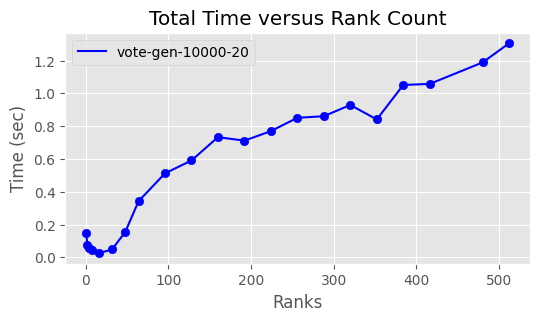
\includegraphics[scale=.6]{../aimos-stats/collection1/plots/vote-gen-10000-20/total_time.png}
\captionof{figure}{Compares the total runtime versus the number of ranks for running
         vote-gen on 10000 voters and 20 candidates. Each point represents an
         actual data point (access
         \href{\repo{aimos-stats/collection1/output/vote-gen-10000-20}}{here})
         collected on AiMOS (DCS) supercomputer. }
\end{center}

Interestingly, the runtime increases as the number of ranks increases, which is
counter to what should happen; more computing power should result in a faster
runtime. However, that is not always the case. The number of candidates is too
small, so the overhead of coordinating a large number of ranks to write to a
file ends up being much more costly than just a smaller number of ranks writing
to a file. In fact, this can be observed in the figure: at first, the run time
dips, but as the number of ranks increases substantially, so does the runtime.
Figure 2 below is still for $m=10000$ and $n=20$, but instead of showing the
total runtime, the runtime for only generating permutations is shown (lines 2
to 4 of the parallel vote generation algorithm).
\begin{center}
    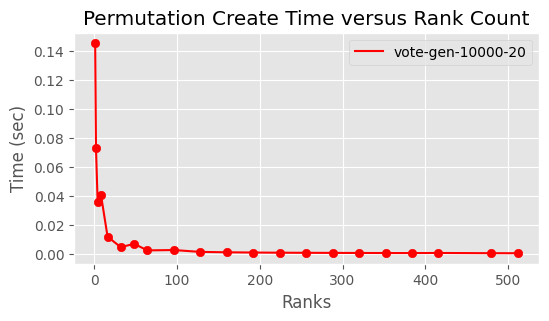
\includegraphics[scale=.6]{../aimos-stats/collection1/plots/vote-gen-10000-20/permutation_create_time.png}
    \captionof{figure}{Compares the permutation generation runtime versus the number of
             ranks for running vote-gen on 10000 voters and 20 candidates. Each
             point represents an actual data point (access
             \href{\repo{aimos-stats/collection1/output/vote-gen-10000-20}}{here})
             collected on AiMOS (DCS) supercomputer. }
\end{center}

Unlike Figure 1, there is a visible decrease in runtime as the number of ranks
increases. This is because the figure does not include the runtimes for writing
to the files, only generating the permutations, suggesting that it is very
relatively expensive to collectively call MPI write operations for all ranks.
However, as the number of candidates and voters increases, I expect the extra
burden from additional coordination MPI ranks to be insignificant. In fact,
looking at Figure 3 below with $m=10^8$ and $n=20$, that exactly is the case.
\begin{center}
    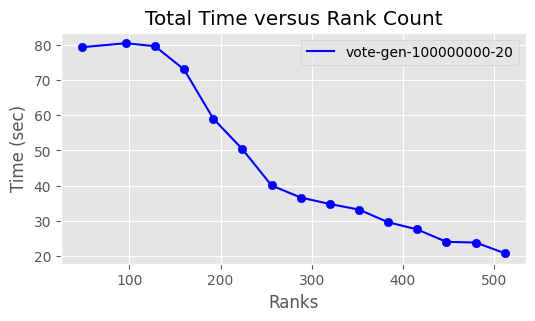
\includegraphics[scale=.6]{../aimos-stats/collection2/plots/vote-gen-100000000-20/total_time.png}
    \captionof{figure}{Compares the total runtime versus the number of ranks for running
             vote-gen on $10^8$ voters and 20 candidates. Each point represents
             an actual data point (access
             \href{\repo{aimos-stats/collection2/output/vote-gen-100000000-20}}{here})
             collected on AiMOS (DCS) supercomputer. }
\end{center}

Here the runtime does indeed decrease as the number of ranks increases. Without
distributing the computing, we would not have been able to generate the file in
a reasonable amount of time. Using only 1 rank was completely insufficient, and
the batch job was canceled over 10 minutes in. In fact, only until 48 ranks
were we able to generate the file with a total runtime of about 3 minutes.
Using 512 ranks reduced the runtime by about 25\% to 40 seconds.

The figure below shows the relationship between vote count and runtime between
a different number of ranks. As already explained above, a large number of
ranks with a low vote count is counterproductive because the overhead cost is
much higher than the I/O cost. Figure 4 below provides some insight as to where
this inflection point occurs number where the cost of overhead overturns I/O.
\begin{center}
    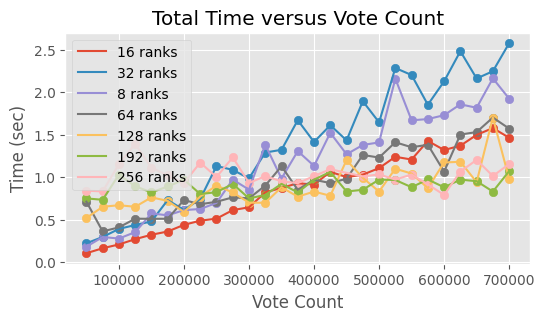
\includegraphics[scale=.6]{../aimos-stats/collection4/plots/total_time.png}
    \captionof{figure}{Compares the total runtime versus the number of votes
             for generating vote file. Each rank has its own line indicated by
             the legend. Each point represents an actual data point (access
             \href{\repo{aimos-stats/collection4/output}}{here}) collected on
             AiMOS (DCS) supercomputer. }
\end{center}

From this figure, we can see that lower number rank counts perform much better
until the vote count reaches $4\times10^5$. After that, higher number rank
counts start to achieve a lower run time. One puzzling thing is that 8 and 16
ranks seem to perform much better than 32 ranks consistently for all vote
counts; we redid this experiment to see if that was a fluke, but 32 ranks still
performed much worse.

Figure 5 below shows the permutation creation time versus vote counts. As
expected, indicated by Figure 1, the higher the rank count, the permutation
creation time will always be lower because there is no I/O time factored in. In
the figure, this is immediately apparent, with 256 ranks runtime consistently
being lower than all the other ranks. However, again, one notable thing is that
32 ranks perform worse than expected, and the same observation was made after
redoing the experiment.
\begin{center}
    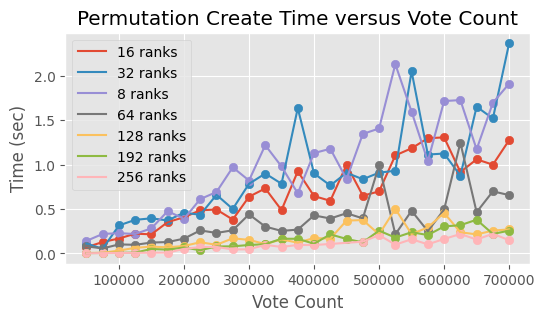
\includegraphics[scale=.6]{../aimos-stats/collection4/plots/permutation_create_time.png}
    \captionof{figure}{Compares the permutation creation time versus the number of votes.
             Each rank has its own line indicated by the legend. Each point
             represents an actual data point (access
             \href{\repo{aimos-stats/collection4/output}}{here}) collected on
             AiMOS (DCS) supercomputer. }
\end{center}

\section{Tallying Votes}
\label{Tallying Votes}

\subsection{Schulze Method and Graph Creation}
\label{Schulze Method and Graph Creation}
The main algorithm we use to create a finalized candidate ranking is the
Schulze method. The algorithm is a graph algorithm, which is similar to the
Floyd-Warshall algorithm in that it compares paths between all pairs of
vertices. As a result, the run time of the algorithm is $O(n^3)$, where $n$ is
the number of candidates \cite{schulze1}. This seems like an issue for scaling
up; however, the number of candidates stays constant and is typically a small
number. As a result, there really is no use in parallelizing this aspect of the
algorithm. Where parallelization comes into play is the actual creation of the
graph, which we represent using an adjacency matrix. The algorithm is given
below:
\begin{algorithm}[H]
    \caption{Preference Graph Generation}\label{alg:cap}
    \begin{algorithmic}[1]
    \Procedure{GraphGen}{$rank$, $startId$, $endId$, $data$}
    \For{$voter\gets startId, endId$}
        \State $ranking = data[voter]$ \Comment{Get candidate ranking.}
        \For{$i\gets 0,$ sizeOf($ranking$)}
            \For{$j\gets i+1,$  sizeOf($ranking$)}
            \State $row \gets ranking[i]$
            \State $col \gets ranking[j]$
            \State $graph[row][col] += 1$
            \EndFor
        \EndFor
    \EndFor
    \State MPIReduce$(graph, finalGraph,$ MPI\_SUM)
    \EndProcedure
    \end{algorithmic}
\end{algorithm}

This algorithm is run on every rank concurrently. Similar to the first the
algorithm in Section 2.2, the same arguments are passed in with the addition of
$data$, which contains all the votes for each voter in the rank's id range. An
example vote is in the form $\{c_1, c_2, c_3, \ldots, c_n\}$, which is passed
to $ranking$ on line 3. $graph$ represents preferences for each candidate such
that $graph[c_i][c_j] = k$ means that $c_i$ is preferred to $c_j$ a total of
$k$ times; note that $k \geq 0$. To generate $graph$, the following is done
from lines 2 to 11: for all $i$ and $j$ where $i < j$, $c_i$ is preferred to
$c_j$, so we increment $graph[c_i][c_j]$ by 1. $graph$ contains all the
pairwise preferences only for the data stored on its own rank, so a reduce the
operation needs to be performed, to sum up all the graphs. This is done on line
12 with \C{MPI_Reduce}, and $finalGraph$ is stored only on rank 0, containing
preferences for the whole vote data set:
\begin{center}
    \begin{BVerbatim}
    MPI_Reduce(graph, final_graph, 
              graph_size, MPI_INT,
              MPI_SUM, 0, MPI_COMM_WORLD);
    \end{BVerbatim}
\end{center}
After generating the final graph, the only step left is to calculate the final
candidate ranking using the Schulze method, which is fairly trivial.
\subsection{Permutation Generation and Monte Carlo}
\label{Permutation Generation and Monte Carlo}
A core requirement of simulating a voting system is being able to generate a
permutation of candidates ($P$), or a vote, according to some distribution that
describes candidate placement relative to one another. $P$ can be generated
efficiently using the Fisher-Yates shuffle algorithm \cite{hazra}; the run time
of the algorithm is linear in the number of candidates, $O(|P|)$. The algorithm
uniformly generates permutations such that given a complete set of $|P|!$
permutations $\mathbf{P} = \{P_1, P_2, P_3, \ldots, P_{|P|!}\}$ each $P_i$ is
equally likely to be generated with probability ${1}/{|\mathbf{P}|}$. Also, if
you look at all the permutations in $P$, for some $i$ and $j$ where $i\neq j$,
the amount of times $c_i$ is preferred to $c_j$ ($c_i >> c_j$) appears in
exactly $|\mathbf{P}|/2$ different permutations. This means that 
\begin{center}
    $\mathbb{E}(c_i >> c_j) = \dsum{i=0}{|\mathbf{P}|/2} \mathds{P}(c_i >> c_j) = \dfrac{1}{2}$.
\end{center}
This has some unique characteristics in regard to the preference graph. This
means that every entry in the graph has an expected value of $m/2$, where $m$
is the number of voters, regardless of the number of candidates. We can use
Monte Carlo to verify this. Using $m=1000000$ and $n=2$ generates the
preference graph: 
\begin{center}
    \scalebox{.9}{
    $ \begin{bmatrix}
        0 & 499315 \\
        500699 & 0
        \end{bmatrix}  $
    }
\end{center}
Using $m=1000000$ and $n=5$ generates the
following preference graph:
\begin{center}
\scalebox{.9}{
$ \begin{bmatrix}
    0 & 500440 & 499949 & 499807 & 500809 \\
    499568 & 0 & 499413 & 499470 & 500436 \\
    500059 & 500595 & 0 & 499703 & 500173 \\
    500201 & 500538 & 500305& 0 & 500224 \\
    499199 & 499572 & 499835 &  499784 & 0 
    \end{bmatrix}  $
}
\end{center}
All the entries for both graphs are approximately $m/2$, and dividing all the
entries by $m$ approximately results in $\frac{1}{2}$.

Instead of uniformly sampling permutations from $\mathbf{P}$, we can apply
different distributions depending on how likely we think one candidate is going
to be preferred to another. Consider the distribution where a candidate $c_i$
is unconditionally preferred to other candidates. That is for a single fixed
candidate $c^*$, $\mathds{P}(c^* >> c_j) = 1$, and consequently,
$\mathbb{E}(c^* >> c_j) = 1$. For all $i$ and $j$ where $i \neq j$ and $c_i
\neq c^*$, $\mathbb{E}(c^* >> c_j) = \frac{1}{2}$. Using $m=1000000$, $n=5$ and
$c^* = 3$ generates the following preference graph and candidate ranking:
\begin{center}
\scalebox{.9}{
$ \begin{bmatrix}
    0& 500147& 0& 499580& 500224 \\
    499861& 0& 0& 499935& 499113 \\
    1000008& 1000008& 0& 1000008& 1000008 \\
    500428& 500073& 0& 0 499800 \\
    499784& 500895& 0& 500208& 0 
\end{bmatrix}$
} \\ 
\vspace*{.2cm}
Ranking: \textbf{3}, 4, 1, 5, 2
\end{center}
As you can see, all the entries except the third row are approximately equal
$m/2$, the third row is approximately equal to $m$, and candidate 3 ranks
first.

The two distributions shown in this section are relatively simple, and their
expected values can easily be computed. However, as the number of candidates
increases, and if the distributions are not exactly trivial, Monte Carlo
simulations may be needed to get preference statistics.

\subsection{Results}
\label{Results2}

Parallelizing the vote tallying algorithm did allow for an increase in
performance as the number of vote counts increased. Similar to the result
analysis in Section 1, using too many ranks on small vote counts ended up being
slower and increased runtimes. However, Figure 6 below indicates that as vote
counts continue to increase, using more ranks is indeed much more beneficial.
In the plot, the inflection point occurs around $8\times 10^5$ votes, and by
$10^6$ votes, the higher ranks do purely better. These results indicate that
our algorithm is well parallelized and will benefit when using significantly
large vote counts.
\begin{center}
    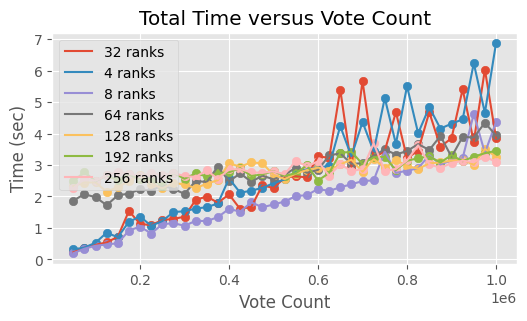
\includegraphics[scale=.6]{../aimos-stats/collection7/plots/total_time.png}
    \captionof{figure}{Compares the total time versus the number of votes for
             generating candidate listings. Each rank has its own line
             indicated by the legend. Each point represents an actual data
             point (access
             \href{\repo{aimos-stats/collection7/output/vote-algo}}{here})
             collected on AiMOS (DCS) supercomputer. }
\end{center}


\section{Encryptin' and Hashin' Votes}
\label{Encrypting and Hashing Votes}

\subsection{Intro to AES}
To encrypt the vote data, we fully implemented the Advanced Encryption Standard (AES) which is the same cipher used by SSL/HTTPS and SSH,
and is one of the most secure encryption algorithms currently available. AES is a block cipher, and typically encrypts 128 bits (or 16 bytes)
at a time. A naive implementation would just encrypt block by block, but this would mean that the same plaintext (or input) would produce the same
ciphertext (encrypted output). With this approach, attackers could recognize patterns in the encrypted vote data to guess how many votes each candidate has.

To use AES securely, we must choose a ``mode''. A well-known and commonly used mode is ``Cipher Block Chaining'' (CBC), where we XOR each input
block with the previous block's ciphertext, using an Initial Vector (IV) for the first block. This ensures that, even if we encrypt identical blocks,
we get completely different resulting ciphertexts. CBC may not be secure if the same input is encrypted twice, but in our case we only encrypt one large
chunk of data a single time. The biggest issue with CBC is that it cannot be parallelized, as the key for each block depends on the previous block.

As AES is expensive, we must use a mode that can be parallelized, such that we can encrypt and decrypt large sums of data as fast as possible. What's more,
the larger the key, the more encryption rounds and thus the more expensive each encryption operation is, thus greatly increasing the running time.

\subsection{AES Counter (CTR) Mode}

AES Counter (CTR) mode is a simple mode whereby we encrypt a ``counter'' block rather than the voting data plaintext itself. The counter block
is typically generated using randomized 96-bits and then a 32-bit unsigned counter to get to the 16 bytes or 128-bit block size required for AES.
Then, for every subsequent 16-byte block, we increment the 32-bit counter which is then encrypted with AES again. With the encrypted counter block,
we can then XOR the plaintext to encrypt the voting data. Because the ``key'' in this case is an AES ciphertext which can be generated just from
the IV and counter value, we can effectively find the XOR key for any block and encrypt/decrypt these blocks independently from each other.

Because the blocks can be independently ciphered, we can parallelize CTR mode and use it to encrypt and decrypt our voting data using threading.
In particular, we can divide up our large voting data file and assign a handful of blocks to each rank, such that each rank has its own chunk of the
larger voting data file, and can use threading to encrypt the smaller blocks in parallel. This means we have two levels of parallelization for AES-CTR
with threading and MPI: multiple threads per rank, and many ranks in the MPI domain.

We use parallel IO to allow each rank to read and write its own set of 128-bit blocks. Because we are working with varying lengths of text, and the
start and end of ``chunks'' of blocks must be deterministic, we pad out the plaintext voting data with hashtag characters to the maximum possible length
of voting strings based on the number of votes and the candidates. This allows deterministic start and end byte positions to be calculated on the
receiving/decrypting side.

\subsection{Intro to SHA-1}

AES grants us confidentiality, but we also need data integrity/authentication to prevent malleability of our encrypted data.
Malleability in cryptography is defined as the degree to which encrypted data can be changed such that an altered plaintext results
when the intended receiver decrypts the data. In particular, it is the possibility to which the modified ciphertext results in a plaintext
that was never encrypted.

To protect against this, we implemented the SHA-1 cryptographic hash. After each rank uses threads to encrypt its share of blocks of voting data,
multi-threaded SHA-1 begins. We define a number of blocks to use for each hash. I.e., we hash every $x$ blocks and append the resulting 20-byte SHA-1
digest to the end of the encrypted data. The receiving side then computes its own hashes over the encrypted data and appends all digests together
together. The large strings of digests are then compared on the receiving side before decryption continues. The hash comparison will now fail if
the encrypting voting data is ever modified by an adversary in transit. 

\subsection{Parallelizing SHA-1}

To multi-thread SHA-1, we simply compute the digests of every $x$ blocks inside each rank, after encryption has completed. With this approach, we again
have two levels of parallelization on the larger voting dataset: each rank computes digests of different smaller chunk of its larger chunk of data from the
voting data, and each rank has a large chunk of the overall data. In our implementation, encryption and hashing is done in the same function, such that
decryption will fail if the hash checks fail. With AES-CTR and SHA-1 combined, we have secure storage of voting data for transmission.

\section{Project Organization}
\label{Project Organization}


\section{Summary and Future Work}
\label{Summary and Future Work}



%% If you have bibdatabase file and want bibtex to generate the
%% bibitems, please use
%%
% \bibliographystyle{elsarticle-harv} 
% \bibliography{example}

%% else use the following coding to input the bibitems directly in the
%% TeX file.

\begin{thebibliography}{20}

\bibitem[Schulze (2018)]{schulze1}
Schulze, M. (2018). The Schulze method of voting. arXiv preprint
arXiv:1804.02973. 
\\
\bibitem[Hazra (2015)]{hazra}
Hazra, T. K., Ghosh, R., Kumar, S., Dutta, S., \& Chakraborty, A. K. (2015,
October). File encryption using fisher-yates shuffle. In 2015 International
Conference and Workshop on Computing and Communication (IEMCON) (pp. 1-7).
IEEE.
\\ 
\bibitem[Schulze (2011)]{schulze2}
Schulze, M. (2011). A new monotonic, clone-independent, reversal symmetric, and
condorcet-consistent single-winner election method. Social choice and Welfare,
36(2), 267-303.
\\
\bibitem[Corbett (1996)]{corbett}
Corbett, P., Feitelson, D., Fineberg, S., Hsu, Y., Nitzberg, B., Prost, J. P.,
Wong, P. (1996). Overview of the MPI-IO parallel I/O interface. Input/Output in
Parallel and Distributed Computer Systems, 127-146.
\\
\bibitem[Pacheco (1997)]{pacheco}
Pacheco, P. (1997). Parallel programming with MPI. Morgan Kaufmann.
\\
\bibitem[Ching (2003)]{ching}
Ching, A., Choudhary, A., Coloma, K., Liao, W. K., Ross, R., and Gropp, W.
(2003, May). Noncontiguous i/o accesses through mpi-io. In CCGrid 2003. 3rd
IEEE/ACM International Symposium on Cluster Computing and the Grid, 2003.
Proceedings. (pp. 104-111). IEEE. \\

\bibitem[Author(year)]{testestestest}
Leslie Lamport (1994) \emph{\LaTeX: a document preparation system}, Addison
Wesley, Massachusetts, 2nd ed.
\\
\bibitem[Author(year)]{testestestest}
Leslie Lamport (1994) \emph{\LaTeX: a document preparation system}, Addison
Wesley, Massachusetts, 2nd ed.
\\
\bibitem[Author(year)]{testestestest}
Leslie Lamport (1994) \emph{\LaTeX: a document preparation system}, Addison
Wesley, Massachusetts, 2nd ed.
\\
\bibitem[Author(year)]{testestestest}
Leslie Lamport (1994) \emph{\LaTeX: a document preparation system}, Addison
Wesley, Massachusetts, 2nd ed.

\end{thebibliography}
\end{document}

\endinput
%%
%% End of file `elsarticle-template-harv.tex'.
